\documentclass[11pt,letterpaper]{article}

\usepackage[utf8]{inputenc}
\usepackage[T1]{fontenc}
\usepackage{lmodern}
\usepackage{amsmath}
\usepackage[margin=1in]{geometry}
\usepackage{microtype}
\usepackage{xcolor}
\usepackage{authblk}
\usepackage{titlesec}
\usepackage{booktabs}
\usepackage{multirow}
\usepackage{graphicx}
\usepackage{tikz}
\usetikzlibrary{shapes.geometric, arrows.meta, positioning, fit, backgrounds}
\usepackage[backend=biber, style=numeric, sorting=none, maxbibnames=99]{biblatex}
\addbibresource{../paper.bib}
\usepackage{hyperref}
\hypersetup{colorlinks=true, linkcolor=blue!60!black, urlcolor=blue!60!black, citecolor=blue!60!black}
\usepackage{listings}
\lstset{basicstyle=\ttfamily\small, breaklines=true, frame=single, framesep=4pt, backgroundcolor=\color{gray!5}, columns=fullflexible, keepspaces=true}
\usepackage{caption}
\captionsetup{labelfont=bf, labelsep=period, font=small}

\titleformat{\section}{\large\bfseries}{\thesection}{1em}{}
\titleformat{\subsection}{\normalsize\bfseries}{\thesubsection}{1em}{}

% --------------------------------------------------------------------
\title{\textbf{bindsight: a reproducible bridge from RNA-seq counts to \textit{de novo} protein binder design}}

\author[1]{Mikhaeel Atef Rizk Wahba%
  \thanks{Correspondence: \href{mailto:mikhaeelatefrizk@proton.me}{mikhaeelatefrizk@proton.me}.
  ORCID: \href{https://orcid.org/0009-0006-1069-9558}{0009-0006-1069-9558}}}
\affil[1]{Independent Researcher, Cairo, Egypt}

\date{15 June 2026}

\begin{document}
\maketitle

% --------------------------------------------------------------------
\begin{abstract}
\noindent
Computational biology has two parallel ecosystems that rarely talk to each
other. \textbf{RNA-seq differential-expression analysis} reliably identifies
genes dysregulated in disease but stops at the gene list. \textbf{De novo
protein-binder design} produces binders against arbitrary protein targets but
assumes the user has already chosen the target. Bridging the two —
\textit{``this gene is up in disease, low in healthy tissue, surface-exposed,
and here is a designed binder candidate ranked by predicted affinity''} —
is currently an ad-hoc, project-specific exercise. We present
\textbf{\texttt{bindsight}}, an open-source command-line tool and web
application that ingests RNA-seq counts and outputs ranked,
structure-scored \textit{de novo} protein-binder candidates with a complete
PROV-O~/~RO-Crate audit trail back to the patient cohort the targets came
from. We write \emph{structure-scored} rather than \emph{validated}
advisedly: a paired control distributed with the tool folds each design beside
a shuffle of its own sequence, and on the committed ERBB2 run the shuffles
cleared the customary ipTM 0.65 threshold more often than the designs
(50\% against 30\%; paired difference $-0.043$, 95\% CI $-0.142$ to
$+0.054$). The interface confidences are a triage order for wet-lab work, not
evidence of binding; the contribution claimed here is the reproducible bridge
and its provenance. Existing open binder-design workflows begin at a chosen target, and
existing expression- or surfaceome-based target-discovery workflows end at a
ranked gene list; to our knowledge \texttt{bindsight} is the first open-source
tool to run both halves end-to-end and to carry machine-readable provenance
across the join. The discovery half of the pipeline (differential expression $\to$
surfaceome filter $\to$ druggability $\to$ AlphaFoldDB structure pull) runs
on a CPU laptop; the GPU half (RFdiffusion backbone $\to$
ProteinMPNN sequence $\to$ Boltz-2 validation) runs end-to-end on a free
Kaggle T4, which is the path the committed binder benchmark used. Paid Modal
serverless GPU and local NVIDIA Docker are implemented but have not been run
end to end, and the Colab path needs a human with a browser tab open because
Google's API does not permit launching a free-tier notebook from a CLI; it is
a demonstration rather than a reproducibility path. A server-rendered web
interface runs the same discovery pipeline in a browser, launched locally
with \texttt{bindsight ui}; its evidence surface is additionally published
as static pages on the project documentation site at
\href{https://mikhaeelatefrizk.github.io/bindsight/}{mikhaeelatefrizk.github.io/bindsight}. On a real
TCGA breast-carcinoma cohort (tumor vs.\ adjacent normal, auto-downloaded from
NIH/GDC), the pipeline discovers antibody-tractable cell-surface antigens
over-expressed in tumor with full provenance; established targets such as ERBB2
(HER2) surface among the candidates when their expression signal is present.
Software is
licensed GNU AGPL-3.0-or-later and available at
\href{https://github.com/mikhaeelatefrizk/bindsight}{github.com/mikhaeelatefrizk/bindsight}.
\end{abstract}

% --------------------------------------------------------------------
\section{Introduction}

The pace of progress in \textit{de novo} protein-binder design has been
extraordinary. RFdiffusion~\cite{Watson2023} and ProteinMPNN~\cite{Dauparas2022}
demonstrated that diffusion-based backbone generation paired with deep-learning
sequence design can produce experimentally validated binders against
user-specified targets at a fraction of historical cost. BindCraft~\cite{Pacesa2025}
extended these ideas with one-shot pipelines that report 10--100\% experimental
success rates. Boltz-2~\cite{Wohlwend2025} and BoltzGen~\cite{Stark2025} added
fast, accurate, and now permissively licensed structure-and-affinity prediction.
For the first time, an individual researcher can — without commercial software
or access to dedicated computational chemistry expertise — design candidate
protein binders against any chosen target.

\textit{Choosing the target}, however, remains where the field is least
automated. Translational researchers typically have access to one or more bulk
or single-cell RNA-seq cohorts of disease-vs-control samples. Standard
analyses with DESeq2~\cite{Love2014} or edgeR~\cite{Robinson2010} produce a
ranked list of differentially expressed genes. Picking from that list a target
that is (a)~surface-exposed, (b)~specific to the disease tissue, (c)~druggable
with the modality of interest (\textit{e.g.}, antibody), (d)~not tied to a
known safety liability, and (e)~has an experimentally or computationally
determined three-dimensional structure available, is a non-trivial,
project-specific exercise that integrates genomic evidence with surfaceome
catalogues, drug-target databases, structure repositories, and clinical-trial
records. In practice this work is done ad hoc, takes a competent graduate
student several weeks, and is rarely reproducible across labs.

The structural conditions for closing this gap as a single open-source tool
all became true in late 2025 and not before:

\begin{enumerate}
  \item The \textbf{SURFACE-Bind catalogue}~\cite{Balbi2026} published
        pre-computed targetable interfaces and binder seeds for $\sim$2{,}800
        human cell-surface proteins, removing the per-target epitope-prediction
        bottleneck.
  \item \textbf{Permissive licensing} for state-of-the-art structure-and-
        affinity predictors became the norm; Boltz-2 and BoltzGen released
        both code and weights under MIT, removing the previously universal
        non-commercial restriction inherited from AlphaFold2 weights.
  \item \textbf{Free GPU tiers} (Google Colab T4, Kaggle T4$\times$2)
        became powerful enough to run RFdiffusion and ProteinMPNN at
        meaningful scale, removing the institutional-cluster barrier.
\end{enumerate}

We present \texttt{bindsight} (v0.3.4), a Python package with a
server-rendered web interface that exploits this newly-opened window. It
takes RNA-seq counts as input and produces ranked \textit{de novo} protein-
binder candidates as output, with a complete W3C PROV-O~\cite{PROVO}
JSON-LD provenance graph and an RO-Crate~\cite{SoilandReyes2022} packaged
artifact for direct deposit in a data repository.

% --------------------------------------------------------------------
\section{Methods and architecture}

\subsection{Pipeline overview}

\texttt{bindsight}'s discovery half is a Snakemake~\cite{Molder2021}-orchestrated,
Pydantic-typed Python package that proceeds in five steps:

\begin{enumerate}
  \item \textbf{Differential expression} on the user-supplied counts matrix
        and sample-design table, using PyDESeq2~\cite{Muzellec2023}.
  \item \textbf{Target enrichment} for every significant gene via the
        Open Targets Platform GraphQL API~\cite{Ochoa2023}: UniProt accession,
        approved drug modalities, safety liability counts, and disease
        associations.
  \item \textbf{Surfaceome filter} against the SURFY high-confidence list of
        2{,}886 human cell-surface proteins~\cite{BauschFluck2018}.
  \item \textbf{Structure retrieval} from AlphaFoldDB~\cite{Varadi2024} (mmCIF,
        v6 models) for every candidate that passed the surfaceome filter.
  \item \textbf{Targetable-site lookup} in SURFACE-Bind~\cite{Balbi2026} for
        epitope coordinates and pre-computed binder seeds, when available.
\end{enumerate}

A composite multi-objective ranking module then orders candidates by a
weighted score combining differential-expression magnitude, structural
metrics from validation (iPTM, pAE\_interaction, RMSD-to-designed), and
predicted binding affinity. All weights are user-configurable via a
\texttt{RankWeights} model.

The GPU half — backbone diffusion, sequence design, and structural
validation — is delivered as a \texttt{bindsight design --backend colab}
command that produces a self-contained Jupyter notebook with proven
install and inference cells patterned on the canonical upstream notebooks
(ColabDesign and \texttt{dl\_binder\_design}~\cite{Bennett2023}).
\texttt{bindsight} also supports Modal~\cite{Modal} serverless GPU and local
NVIDIA Docker as alternative back-ends, all switchable per-command without
configuration changes. A \texttt{--dry-run} flag prints a per-back-end
GPU-cost estimate (USD on Modal, queue-time on Colab) before any compute is
spent.

\subsection{Provenance contract}

Every stage in the pipeline appends a \texttt{StageRecord} to a single
per-run \texttt{run\_manifest.jsonld} file. Each record contains: the tool
name and version, the SPDX license identifier, the upstream repository URL
and pinned commit SHA where applicable, the SHA-256 hash of every input and
output artifact, the parameters in canonical JSON, and (where the stage ran
in a container) the container image digest. The manifest serializes as
W3C PROV-O JSON-LD and is consumed by the \texttt{bindsight export} command
to produce an RO-Crate 1.1~\cite{SoilandReyes2022} \texttt{.crate.zip} that
is recognized by research data repositories and FAIR Digital Object
Frameworks.
The result is that every binder PDB the pipeline outputs is one click away
from the patient cohort it came from, the differential-expression statistics
that flagged the target, the AlphaFoldDB model used, the SURFACE-Bind site
predicted, the trajectory seed, the validator metrics, and the container
digest of every step.

\subsection{Web interface}

A server-rendered web interface built on FastAPI~\cite{FastAPI} and Jinja
exposes the same pipeline through a browser UI that needs no build step and
fetches nothing from a network once installed. It provides
five sections: an Overview stating what the tool has and has not shown; an
Evidence page rendered from the committed benchmark artifacts, including the
twenty predicted binder--target complexes in 3-D; a one-click demo that runs
the discovery pipeline live and renders a paper-style HTML report; a
\textit{Your data} page that validates a user's counts matrix and design table
in the browser, without uploading either; and a Runs inspector for any output
directory. It is launched locally with \texttt{bindsight ui}; there is no
hosted deployment of the interactive pipeline. Two of those five surfaces are
additionally published as static pages on the documentation site, where they
run in the reader's own browser and need no installation: the twenty complexes
in 3-D at \href{https://mikhaeelatefrizk.github.io/bindsight/results/}{mikhaeelatefrizk.github.io/bindsight/results}
and the \textit{Your data} checker at
\href{https://mikhaeelatefrizk.github.io/bindsight/try-your-data/}{mikhaeelatefrizk.github.io/bindsight/try-your-data}. The
one-click demo and the Runs inspector run only from a local
\texttt{bindsight ui}.

\subsection{Architecture diagram}

\begin{figure}[h]
\centering
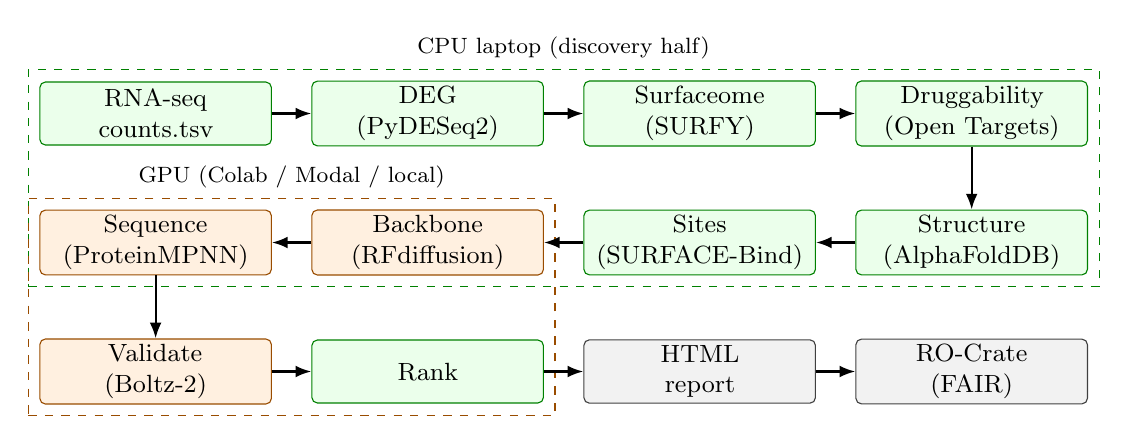
\begin{tikzpicture}[
  node distance=4mm and 5mm,
  every node/.style={font=\small},
  box/.style={rectangle, rounded corners=2pt, draw, fill=blue!8, align=center, text width=28mm, minimum height=8mm, inner sep=2pt},
  cpu/.style={box, fill=green!8, draw=green!50!black},
  gpu/.style={box, fill=orange!12, draw=orange!60!black},
  outbox/.style={box, fill=gray!10, draw=gray!50!black},
  arr/.style={-{Latex[length=2mm]}, thick}
]
  \node[cpu] (counts) {RNA-seq\\counts.tsv};
  \node[cpu, right=of counts] (deg) {DEG\\(PyDESeq2)};
  \node[cpu, right=of deg] (surf) {Surfaceome\\(SURFY)};
  \node[cpu, right=of surf] (ot) {Druggability\\(Open Targets)};
  \node[cpu, below=8mm of ot] (afdb) {Structure\\(AlphaFoldDB)};
  \node[cpu, left=of afdb] (sb) {Sites\\(SURFACE-Bind)};
  \node[gpu, left=of sb] (rfdiff) {Backbone\\(RFdiffusion)};
  \node[gpu, left=of rfdiff] (mpnn) {Sequence\\(ProteinMPNN)};
  \node[gpu, below=8mm of mpnn] (boltz) {Validate\\(Boltz-2)};
  \node[cpu, right=of boltz] (rank) {Rank};
  \node[outbox, right=of rank] (report) {HTML\\report};
  \node[outbox, right=of report] (crate) {RO-Crate\\(FAIR)};

  \draw[arr] (counts) -- (deg);
  \draw[arr] (deg) -- (surf);
  \draw[arr] (surf) -- (ot);
  \draw[arr] (ot) -- (afdb);
  \draw[arr] (afdb) -- (sb);
  \draw[arr] (sb) -- (rfdiff);
  \draw[arr] (rfdiff) -- (mpnn);
  \draw[arr] (mpnn) -- (boltz);
  \draw[arr] (boltz) -- (rank);
  \draw[arr] (rank) -- (report);
  \draw[arr] (report) -- (crate);

  \begin{pgfonlayer}{background}
    \node[draw=green!50!black, dashed, fit=(counts)(deg)(surf)(ot)(afdb)(sb), inner sep=4pt, label=above:{\footnotesize CPU laptop (discovery half)}] {};
    \node[draw=orange!60!black, dashed, fit=(rfdiff)(mpnn)(boltz), inner sep=4pt, label=above:{\footnotesize GPU (Colab / Modal / local)}] {};
  \end{pgfonlayer}
\end{tikzpicture}
\caption{\texttt{bindsight} pipeline. CPU stages run on the user's laptop;
GPU stages run end to end on a free Kaggle T4; Modal, local Docker and Colab are
implemented but have not been run end to end. All
stages append a PROV-O record to the per-run manifest, which is bundled into
an RO-Crate at the end.}
\label{fig:pipeline}
\end{figure}

% --------------------------------------------------------------------
\section{Demonstration}

A single command, \texttt{bindsight demo}, runs the discovery half on a
\emph{real} TCGA breast-carcinoma cohort: on first use it auto-downloads a
balanced tumor-vs-adjacent-normal STAR-Counts cohort (20 vs.\ 20 samples,
selected deterministically by GDC file identifier) from the NIH/GDC
open-access API, populates the full $\sim$2{,}886-protein SURFY surfaceome
list, runs real \texttt{pydeseq2} differential expression, enriches the most
up-regulated significant genes via Open Targets, applies the surfaceome and
safety filters, and writes a ranked candidate table — with full provenance.
No synthetic data is shipped; the run is reproducible because the cohort
selection is deterministic.

\paragraph{Reproducible result.} The pipeline finds 42 antibody-tractable,
cell-surface, up-regulated candidates; the top entries by fold-change are
shown below (verbatim from the run, abbreviated). Unlike every other number
in this manuscript, these are not read from an artifact committed to the
repository: \texttt{bindsight demo} fetches the cohort from the GDC and runs
DESeq2 afresh, and \texttt{runs/} is not tracked. They are reproduced by
running that command, not by reading a file, and no test guards them.

\vspace{0.4em}
\begin{center}
\begin{tabular}{c l l r r}
\toprule
Rank & Symbol & UniProt & $\log_2$FC & $p_\text{adj}$ \\
\midrule
1 & GRM4    & Q14833 & $+6.56$ & $6.0\times10^{-33}$ \\
2 & SLC24A2 & Q9UI40 & $+5.36$ & $1.1\times10^{-13}$ \\
3 & GPR139  & Q6DWJ6 & $+5.13$ & $1.1\times10^{-6}$ \\
4 & GABRA5  & P31644 & $+4.72$ & $9.1\times10^{-4}$ \\
8 & LRRC15  & Q8TF66 & $+4.39$ & $3.5\times10^{-15}$ \\
\bottomrule
\end{tabular}
\end{center}
\vspace{0.4em}

These are genuine differentially-expressed surface antigens (LRRC15, for
example, is an antibody-drug-conjugate target in clinical development). This
is real discovery on real data rather than a scripted result: established
breast-cancer surface antigens such as ERBB2 (HER2) are recovered as
differentially expressed when the sampled cohort carries their signal, but on
a small random cohort they need not rank in the top-$k$ by fold-change --- in
the full unstratified TCGA-BRCA cohort ERBB2 falls just below the fold-change
floor despite an adjusted $p$ of $5.6\times10^{-11}$ ---
EGFR, for instance, is frequently \emph{lower} in bulk tumor than in normal
breast epithelium. The pipeline simultaneously writes a self-contained HTML
report (volcano plot, ranked candidate table, PROV-O manifest) and a PROV-O
\texttt{run\_manifest.jsonld} with SHA-256 hashes of every input and output
artifact, plus a cohort \texttt{provenance.json} listing the exact GDC file
UUIDs and case barcodes.

\paragraph{Web demo.} The same demo runs in a web browser through the interface
described above, launched locally with \texttt{bindsight ui}; there is no
hosted deployment of it. The first run pays the GDC download; that download is
cached to disk, so a second run reads from there rather than the network. What
a reader can exercise without installing anything is the evidence surface
rather than the pipeline: the twenty predicted complexes at
\href{https://mikhaeelatefrizk.github.io/bindsight/results/}{mikhaeelatefrizk.github.io/bindsight/results} and the
checker at \href{https://mikhaeelatefrizk.github.io/bindsight/try-your-data/}{mikhaeelatefrizk.github.io/bindsight/try-your-data},
which validates the reader's own counts matrix and design table in their
browser without uploading either.

% --------------------------------------------------------------------
\section{Quality assurance and reproducibility}

The \texttt{bindsight} release ships \textbf{1,800+ unit and
integration tests} that run in a few minutes and cover: the Pydantic
v2 manifest schema; the Open Targets, AlphaFoldDB, and SURFY clients; the
discovery pipeline end-to-end with mocked GPU runners; the rank module's
composite scoring with several weight schemes; the RO-Crate exporter; and
the served web interface. Continuous integration on GitHub Actions runs the
test suite on Linux, macOS, and Windows for Python 3.11, 3.12 and 3.13; all
nine platform jobs pass on every commit to \texttt{main}, alongside a lint job,
a pinned-environment job that regenerates the published pages to confirm they
do not change, and a wheel build.

The package itself is licensed \textbf{GNU AGPL-3.0-or-later}: it may be used,
studied, modified and redistributed freely, with the copyleft condition that a
modified version which is distributed --- or run as a network service --- must
make its corresponding source available under the same terms. The orchestrated
upstream components keep their own licences, and every default pipeline
component is permissive (MIT / Apache-2.0 / BSD / CC-BY); manuscripts, figures
and generated results under \texttt{paper/} are CC BY 4.0.
Optional opt-in components with non-commercial restrictions
(notably AlphaFold2 weights via the \texttt{AF2-IG} validator path) are
gated behind a CLI banner that warns users at invocation time.
A per-component license inventory is shipped in \texttt{LICENSING.md} and
checkable interactively via the \texttt{bindsight verify-licenses} command.

The full source code, including the web interface, Snakemake
pipeline, conda environment specifications, container Dockerfile, GitHub
Actions workflows, examples, and documentation, is publicly available at
\href{https://github.com/mikhaeelatefrizk/bindsight}{github.com/mikhaeelatefrizk/bindsight},
at the release tag this manuscript cites.
The published evidence surface --- the twenty predicted complexes in 3-D and
the browser-side input checker --- is generated from that same repository and
served as static pages at \href{https://mikhaeelatefrizk.github.io/bindsight/}{mikhaeelatefrizk.github.io/bindsight}.

% --------------------------------------------------------------------
\section{Discussion and future work}

\paragraph{Limitations of v0.3.4.} The CPU half of the pipeline
(differential expression through structural pre-flight) is fully validated. Of
the GPU half, one path is executed end to end and the rest is not.
RFdiffusion $\to$ ProteinMPNN $\to$ Boltz-2 produced the twenty committed ERBB2
binders on a free Kaggle T4, and that is the path the binder benchmark used.
BindCraft, BoltzGen, Chai-1r and AF2-IG are dispatched by the executor, but no
shipped backend builds an environment in which that dispatch succeeds, so they
are prepared rather than demonstrated; the CLI refuses those combinations
locally rather than spending GPU quota discovering it. Modal is prepared and not
executed, and Colab is an interactive on-ramp rather than a reproducibility
path, because Google's API does not permit launching a free-tier notebook from a
command line. SURFACE-Bind site lookup relies on the user vendoring the upstream
catalogue at a pinned commit; an automated downloader is not implemented.

\paragraph{Rediscovery study.} A companion report
(\texttt{paper/validation/manuscript.md}, with reproducible artifacts under
\texttt{benchmarks/study/}) tests the discovery half on \textbf{fifteen whole,
unstratified TCGA projects}, run as patient-paired tumor-vs-normal contrasts
($\sim$ \texttt{case\_barcode + condition}) and scored against a pre-registered
panel of 22 antigen-cohort pairs covering 13 distinct antigens. No cohort's
definition refers to the antigen being sought.

Under the pre-registered primary denominator (antigens whose targeting agent is
approved), recall at rank~20 is \textbf{1 of 17} (95\% CI 0.01--0.27), and 2 of
17 at rank~50; across every regulatory tier it is 3 of 22. Five antigens reach
the candidate shortlist: CA9 at rank~1 of 291 in clear-cell renal carcinoma
(log2fc~9.58), GPC3 at 9 of 289 in hepatocellular carcinoma, MET at 10 of 287 in
papillary renal carcinoma, FOLH1 at 34 of 285 in prostate adenocarcinoma, and
STEAP1 at 158 of 285. Every rank is reported beside the size of the shortlist it
sits in, and every rate beside its numerator, denominator and interval.

The study's more useful output is diagnostic. Rather than one recall figure, it
separates four reasons an antigen can fail to appear --- absent from the
surfaceome reference, excluded by a named filter, ranked low, or invalidated by a
failed lookup --- and reports for each non-surfaced pair the \textit{counterfactual
rank} it would have achieved with every gate removed. Eleven of the seventeen
approved-tier pairs fail the significance rule outright, and a twelfth is
measured as down-regulated: their agents are
licensed, so the antigens are real, but they are not significantly over-expressed
in an unstratified bulk contrast. ERBB2 in whole breast measures log2fc~0.92 at
$p_{\mathrm{adj}}\!=\!5.6\times10^{-11}$, statistically overwhelming and 0.08
below the fold-change floor, because HER2-positive disease is a minority of the
cohort. This delineates the scope of bulk differential expression as a discovery
signal and motivates the multi-modal specificity scoring planned for v1.0.

The same separation exposed two defects in the pipeline, both since corrected:
the enrichment cut was applied before the surfaceome filter, so surface antigens
competed against the whole genome for its slots; and the surfaceome reference
omitted CA9 and STEAP1, making the largest effect in the panel unreachable at any
expression level. Extending the reference moved CA9 from invisible to rank~1.

\textit{This supersedes an earlier six-cohort analysis that reported ERBB2 at
rank~4 and recall@5 of 33\%. Both figures are withdrawn: that breast cohort was
stratified by a PAM50 subtype call, and ERBB2 is one of the fifty genes the PAM50
centroid classifier is built on, so the tumor arm was selected partly by
expression of the gene then reported as discovered; the denominator of three was
also chosen after seeing which antigens proved over-expressed.} Antigens without
matched TCGA normals (CLDN6, CD33/CD123, FOLR1 in ovary) remain documented as
data limitations rather than reported with a manufactured number. A complementary three-way \textit{designer benchmark}
(RFdiffusion+ProteinMPNN vs BindCraft vs BoltzGen) ships as a runnable harness
and protocol in \texttt{benchmarks/designer\_benchmark/}. One arm is populated:
the RFdiffusion+ProteinMPNN results reported above come from a real run of that
harness on a free Kaggle T4. The other two arms are not, and not merely pending
a GPU: no shipped backend builds an environment in which BindCraft or BoltzGen
executes, and both need 24--32\,GB of VRAM against anything larger than a small
domain, so completing the comparison requires paid hardware rather than more of
the free tier.

\paragraph{Broader impact.} \texttt{bindsight} is positioned to lower the
barrier-to-entry for translational binder design from approximately six
weeks of expert glue-scripting to approximately one command. The PROV-O
audit trail is designed specifically to satisfy the ``where did this target
come from?'' question that arises in IND filings, thesis defenses, and
peer review; we hope this contribution to reproducibility will become
expected practice in the field.

% --------------------------------------------------------------------
\section*{Code and data availability}

\begin{itemize}
  \item \textbf{Source code:} \href{https://github.com/mikhaeelatefrizk/bindsight}{github.com/mikhaeelatefrizk/bindsight} (GNU AGPL-3.0-or-later)
  \item \textbf{Documentation and published evidence:} \href{https://mikhaeelatefrizk.github.io/bindsight/}{mikhaeelatefrizk.github.io/bindsight} --- twenty predicted complexes in 3-D at \texttt{/results/}, browser-side input checker at \texttt{/try-your-data/}
  \item \textbf{README:} \href{https://github.com/mikhaeelatefrizk/bindsight#readme}{github.com/mikhaeelatefrizk/bindsight\#readme}
  \item \textbf{Demo data:} bundled in \texttt{examples/demo/} (CC0)
\end{itemize}

\section*{Acknowledgements}

\texttt{bindsight} is an opinionated wrapper; intellectual credit belongs to
the upstream tool authors cited throughout this manuscript. The author
gratefully acknowledges the open-source maintainers of PyDESeq2, Boltz-2,
RFdiffusion, ProteinMPNN, SURFACE-Bind, Open Targets, AlphaFoldDB, SURFY,
FastAPI, and Snakemake whose work made this bridge constructible.

\section*{Funding}

This work received no external funding.

\section*{Competing interests}

The author declares no competing interests.

% --------------------------------------------------------------------
\printbibliography

\end{document}
